\documentclass[12pt]{article}
\setlength{\oddsidemargin}{0in}
\setlength{\evensidemargin}{0in}
\setlength{\textwidth}{6.5in}
\setlength{\parindent}{0in}
\setlength{\parskip}{\baselineskip}

\usepackage[all]{xy}

\usepackage{amsmath,amsfonts,amssymb}
\usepackage{graphicx}
\usepackage{fancyhdr}
\pagestyle{fancy}
\usepackage{hyperref}

\begin{document}

\lhead{{\bf CSCI 3104 \\ Problem Set 9} }
\rhead{Name: \fbox{Maura Kieft} \\ ID: \fbox{103947905} \\ {\bf Profs.\ Grochow \& Layer\\ Spring 2019, CU-Boulder}}
\renewcommand{\headrulewidth}{0.5pt}
\phantom{Test}

Quick links \ref{1a} \ref{1b} \ref{1c} \ref{1d} \ref{2} \ref{3}


\vspace{-3mm}
\begin{enumerate}

	\item (30 pts) Bidirectional breadth-first search is a variant of standard BFS for finding a shortest path between two vertices $s,t \in V(G)$. The idea is to run \emph{two} breadth-first searches simultaneously, one starting from $s$ and one starting from $t$, and stop when they ``meet in the middle'' (that is, whenever a vertex is encountered by both searches). ``Simultaneously'' here doesn't assume you have multiple processors at your disposal; it's enough to alternate iterations of the searches: one iteration of the loop for the BFS that started at $s$ and one iteration of the loop for the BFS that started at $t$.
	
	As we'll see, although the worst-case running time of BFS and Bidirectional BFS are asymptotically the same, in practice Bidirectional BFS often performs significantly better.
	
	Throughout this problem, all graphs are unweighted, undirected, simple graphs.
	
	\begin{enumerate}
	\item \label{1a} (5 pts) Give examples to show that, in the worst case, the asymptotic running time of bidirectional BFS is the same as that of ordinary BFS. Note that because we are asking for asymptotic running time, you actually need to provide an infinite family of examples $(G_n, s_n, t_n)$ such that $s_n,t_n \in V(G_n)$, the asymptotic running time of BFS and bidirectional BFS are the same on inputs $(G_n, s_n, t_n)$, and $|V(G_n)| \to \infty$ as $n \to \infty$.
	% YOUR SOLUTION HERE
	\\
	\\
	The bidirectional BFS is two searches. One from start$(s)$ to the goal, and the second is from goal$(t)$ to the start. The search terminates whenever a vertex is encountered by both searches, meeting in the middle. When finding a source vertex s to a target vertex t, assuming that there is a steady branching factor b, the running time and number of possibilities checked is dependent on the depth. In ordinary BFS, the depth is the distance to the target. Which gives $b^{k}$ vertices visited, giving the asymptotic run time of (1 + b + $b^{2}$ + ... + $b^{d}$ = $\theta(b^{d}$) For bidirectional BFS, the searches meet in the middle. So there is two searches on the depth, making the asymptotic runtime 2 $*$ (1 + b + $b^{2}$ + ... + $b^{d/2}$ = O($b^{d/2}$ where b is the branching factor, and d is depth. \\
	\\For example, if we had the following; \\
 

	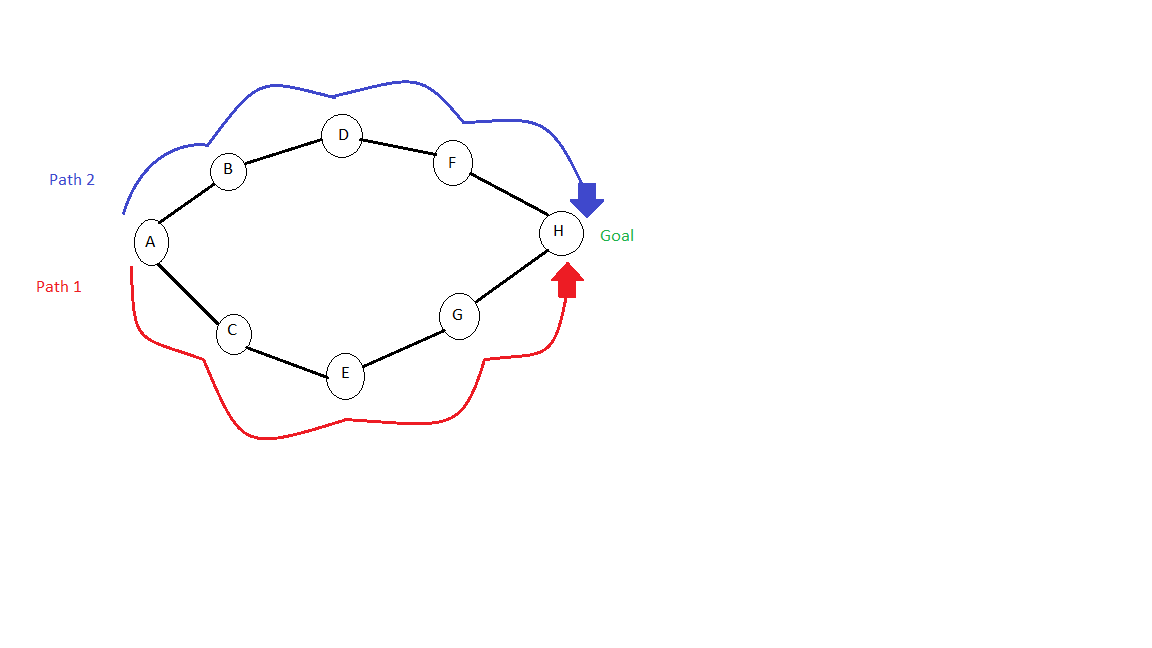
\includegraphics[scale = 0.7]{bidirectional-example.png}
	
	Best case: \\
	In the first search, (A) is the start node and (H) is the goal node. \\	In the second search, (H) is the start node and (A) is the goal node. \\
	So, the first follows the path A - C - E - G - H. \\
	The second search follows the reverse of this, H - G - E - C - A.
	\\ Thus, in this case, both searches meet in the middle. Making the time complexity O($b^{d}$ + $b^{d}$) = O($b^{d}$) \\ \\
	 Worst case: \\
	 The first search chooses the path A - C - E - G - H and the second search chooses the path H - F - D - B - A. Which is the reverse of path 2. Since the first search follows path 1 and the second follows the reverse of path 2, both searches will not ever meet because the follow a different path and will only terminate when both searches encounter the same vertex. Thus, our time complexity for our first search of bidirectional BFS is O(1 + b + $b^{2}$ + $b^{d}$)= O($b^{d}$ and for the second search it is the same, = O($b^{d}$). Which makes a total of O($b^{d} + b^{d}$) = O($b^{d}$) which is the same as that of ordinary BFS.   
	
	\pagebreak
	
	\item \label{1b} (5 pts) Recall that in ordinary BFS we used a \texttt{visited} array (see Lecture Notes 8) to keep track of which nodes had been visited before. In bidirectional BFS we'll need \emph{two} \texttt{visited} arrays, one for the BFS from $s$ and one for the BFS from $t$. Let ``naive bidirectional BFS'' denote an attempted implementation of bidirectional BFS which uses only one {\tt visited} array.  Give an example to show what can go wrong if there's only one \texttt{visited} array. More specifically, give a graph $G$ and two vertices $s,t$ such that some run of a naive bidirectional BFS says there is no path from $s$ to $t$ when in fact there is one.\\
	% YOUR SOLUTION HERE
	\\ When using one visited array to implement the bidirectional BFS, initially all vertices in the array are set to false. The first search is performed from start(s), and if a vertex isn't marked as visited when it is processed, it is added to the first queue(lets say Q1). The second search is performed from the goal(t), and if a vertex isn't marked as visited when it is processed, it is added to the second queue (lets say Q2). So if we were to perform the naive bidirectional BFS on the following;
	
	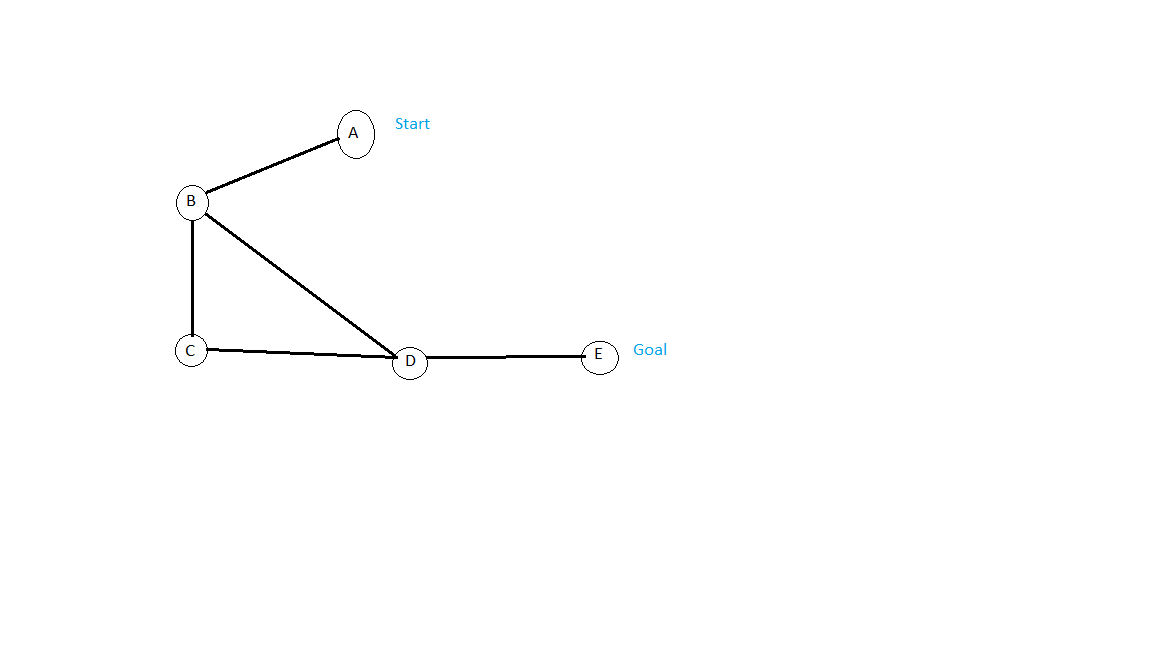
\includegraphics[scale = 0.7]{visitedarrayexample.png}
	
	Initially, all of the vertices in the visited array will be set to false. We have Q1 processing all of the vertices from the start(s) to the goal(t), and Q2 processing all of the vertices from the goal(t) to the start(s). For path 1 beginning at the start(s), vertex A, we look at its adjacent vertices, in this case, it is B. B has not been visited before so B is set to visited[B] = true and added to Q1. For path 2, it begins at the goal(t), which is E. Its adjacent vertex is D, so D is set to visited[D] = true and added to Q2. Continuing with this, looking at the vertices adjacent to B, we find vertex C and mark it as visited[C] = true and add it to Q1. When looking at vertice adjacent to D for the second path, both B and C have already been marked as visited in the visited array, so D does not acknowledge a path to either of the vertices. Thus, when using one visited array in the bidirectional BFS for this example, Q1 would have a path of A - B - C and Q2 would have a path of E - D, which shows that there is no path from the starting vertex (s) to the goal vertex(t), when, in fact, there is one. 
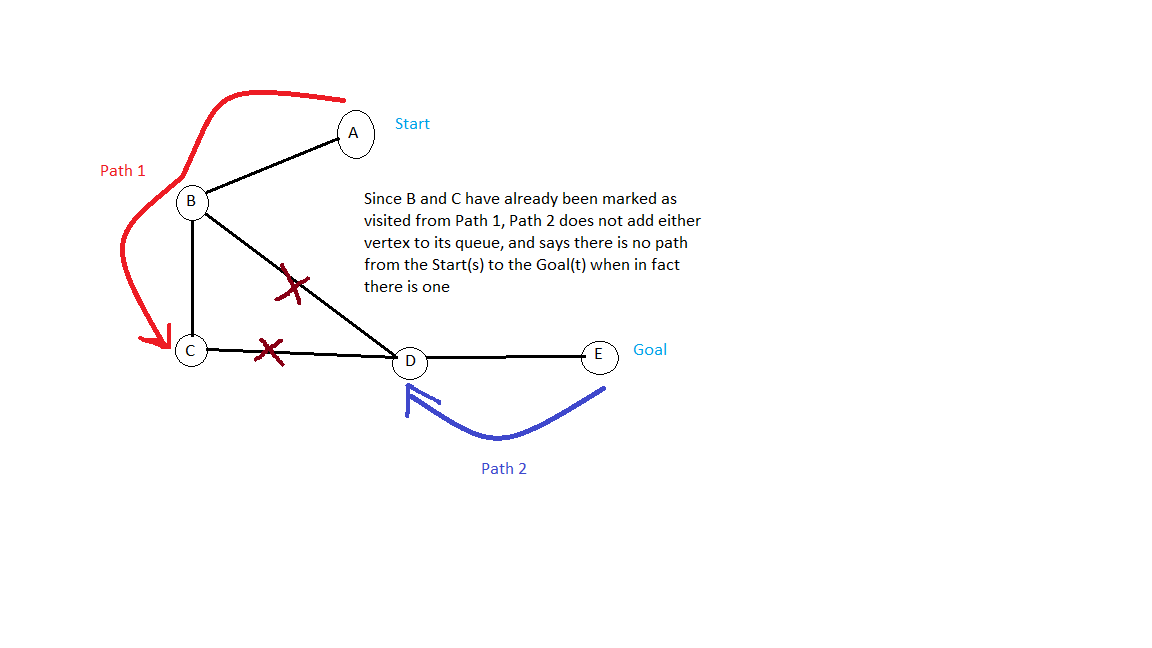
\includegraphics[scale = 0.7]{visitedarrayexample2.png}
	
			
	\pagebreak
	
	\item \label{1c} Consider BFS vs. bidirectional BFS on grids. Namely, let $G_n$ be an $n \times n$ grid, where each vertex is connected to its neighbors in the four cardinal directions (N,S,E,W). Vertices on the boundary of the grid will only have 3 neighbors, and corners will only have 2 neighbors. Let $s_n$ be the midpoint of one edge of the grid, and $t_n$ the midpoint of the opposite edge. For example, for $n=3$ we have:
	
	\[
\xymatrix{
\bullet \ar@{-}[r] \ar@{-}[d] & \bullet \ar@{-}[r] \ar@{-}[d] & \bullet \ar@{-}[d] \\ 
s_3 \ar@{-}[r] \ar@{-}[d] & \bullet \ar@{-}[r] \ar@{-}[d] & t_3 \ar@{-}[d] \\ 
\bullet \ar@{-}[r] & \bullet \ar@{-}[r] & \bullet
}
\]

	\begin{enumerate}
	\item (5 pts) Give an argument as to why BFS starting from $s_n$ searches nearly the entire graph (in fact, a constant fraction of it) before encountering $t_n$. \\
	% YOUR SOLUTION HERE
	\\A breadth first search traverses a graph from the start node, $s{n}$ and then explores all of its neighboring vertices at the present depth before moving onto the nodes at the next depth level. Since $s{n}$ is the midpoint of one edge of the grid, it has 3 "neighbors." After processing these 3 neighbors it moves onto the next depth level of which the first vertex has only one adjacent vertex it will process. The next has only one adjacent vertex it will process. And the next has 3 adjacent vertices, but 2 of them had already been visited, so it ends up processing $t{n}$. Since the graph is of grid like nature, BFS starting from $s{n}$, or the midpoint of one edge of the grid, it searches nearly the entire graph before encountering $t{n}$ because it is a breadth first traversal and it goes one depth at time, exploring almost all of the graph before it gets to the depth of $t{n}$. \\

	\pagebreak
	
	\item (5 pts) Bidirectional BFS also searches a constant fraction of the entire graph before finding a path from $s_n$ to $t_n$, but a smaller constant fraction than ordinary BFS. Estimate this constant, and give an argument to justify your estimate. Hint: as $n \to \infty$, if you ``zoom out'' the graph starts to look more like the unit square $[0,1] \times [0,1]$ in the real plane $\mathbb{R}^2$. Consider the ``spreading'' picture of BFS / bidirectional BFS and use basic geometric facts.
	\end{enumerate}
	% YOUR SOLUTION HERE
	 I don't know. 
	\pagebreak
	
	\item \label{1d} Consider BFS vs. bidirectional BFS on trees. Let $T_n$ is a complete binary tree of depth $n$. $s_n$ is the root and $t_n$ is any leaf. For example, for $n=3$ we have:
	\[
	\xymatrix{
 	   & & & s_3 \ar@{-}[lld] \ar@{-}[rrd] \\ 
	  & \bullet \ar@{-}[dr] \ar@{-}[dl] & & & & \bullet \ar@{-}[dr] \ar@{-}[dl] \\
	\bullet & & \bullet & & t_3 & & \bullet
	}
	\]
	
	\begin{enumerate}
	\item (5 pts) Prove the asymptotic running time of BFS on $T_n$ starting at $s_n$, where the BFS can stop as soon as it finds a path from $s_n$ to $t_n$.\\
	% YOUR SOLUTION HERE
	\\$T{n}$ = complete binary tree \hspace*{10mm} n = depth of $T{n}$ \\$s{n}$ = root \hspace*{20mm} $t{n}$ = any leaf \\
	\\Theorem: The asymptotic running time of BFS on $T{n}$ is O($b^{n-1}$) where b is the branching factor, and n is the depth of the complete binary tree. \\
	\\ Since the starting vertex, $s{n}$ is the root of the tree, and the tree is a complete binary tree, it begins at depth 1 and finds all of its adjacent vertices. It continues this for the next depth, and on until it finds the target leaf node $t{n}$. Since it is a complete binary tree, it does not have to continue onto depth of n, because at depth n-1 the algorithm will find the target vertex and will stop when it reaches it.\\
	For example: \\
	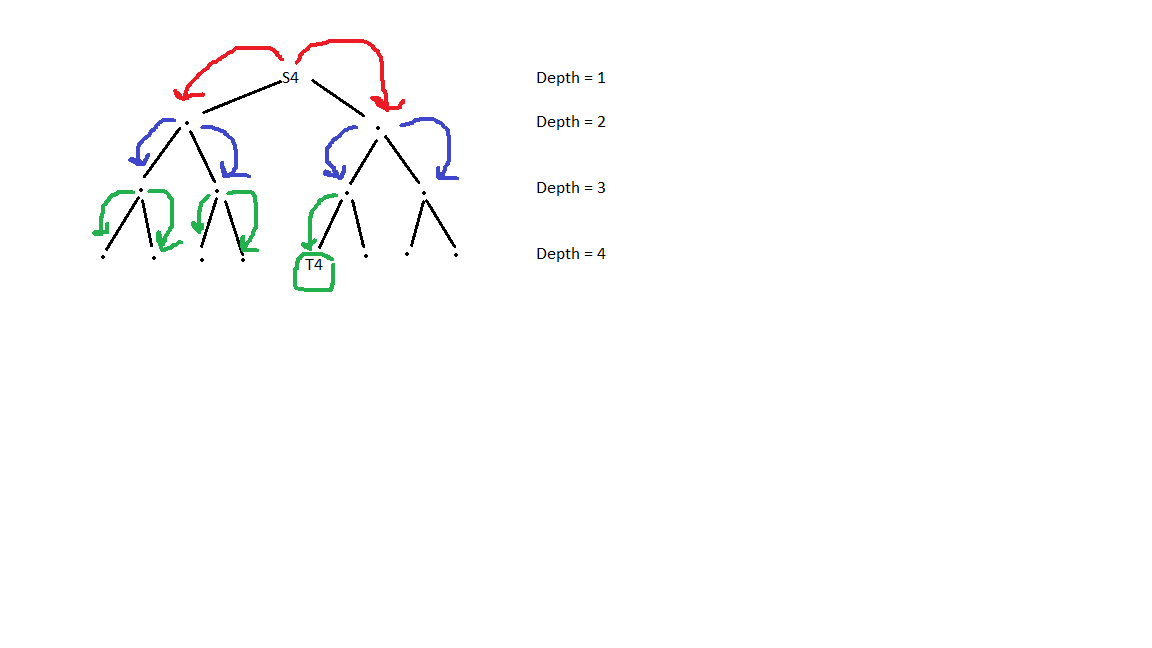
\includegraphics[scale = 0.5]{bfstime.png}
		
	 So, the asymptotic runtime is (1 + b + $b^{2}$ + ... + $b^{n-1}$) = O($b^{n-1}$) 
	
	
	
	 
	 
	\pagebreak

	\item (5 pts) Prove the asymptotic running time of bidirectional BFS on $T_n$ starting at $(s_n, t_n)$.
	% YOUR SOLUTION HERE 
	\\
	\\Theorem: The asymptotic runtime of bidirectional BFS on the complete binary tree $T{n}$ starting at ($s{n}, t{n}$) is O($b^{n-2}$)\\
\\The first path of the bidirectional search begins at the start vertex $s{n}$ and goes to the goal(t). The second path of the bidirectional search begins at the goal $t{n}$ and goes to the start(s). Since $T{n}$ is a complete binary tree, and n is the depth of the tree, both searches begin at their perspective depths and search down, in the case of the first path, and up, in the case of the second path. Both searches, in theory, should cut the depth in half, but because of the complete binary tree it may take a while to traverse to each other by depth. Eventually, both paths will meet to complete the bidirectional BFS at n-2. 
For example, \\
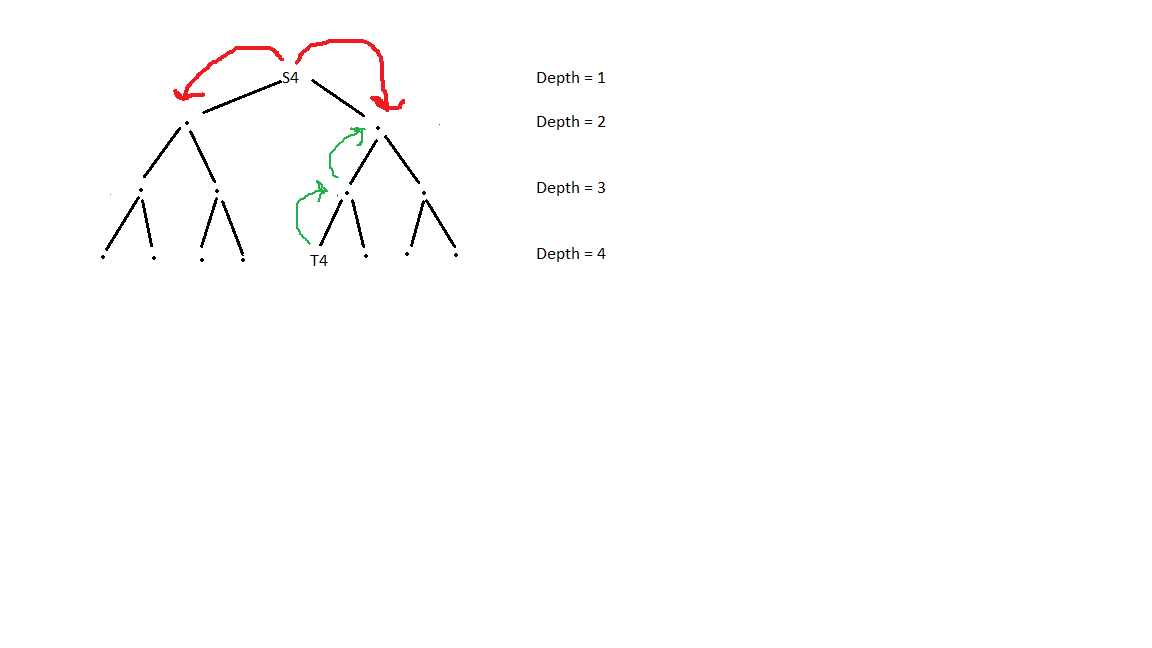
\includegraphics[scale = 0.5]{bfstime2.png}
Thus, the asymptotic run time of bidirectional BFS on $T{n}$ starting at ($s{n}, t{n}$) is (1 + b + $b^{2}$ + ... + $b^{n-2}$) = O($b^{n-2}$)
	\pagebreak
	
	\end{enumerate}		
	\end{enumerate}
	

	\item \label{2} (10 pts) Let $G=(V,E)$ be a graph with an edge-weight function $w$, and let the tree $T\subseteq E$ be a minimum spanning tree on $G$. Now, suppose that we modify $G$ slightly by decreasing the weight of exactly one of the edges in $(x,y)\in T$ in order to produce a new graph $G'$. Here, you will prove that the original tree $T$ is still a minimum spanning tree for the modified graph $G'$. \\
	 To get started, let $k$ be a positive number and define the weight function $w'$ as
%
\begin{displaymath}
w'(u,v) = \left\{
\begin{array}{ll}
w(u,v) & \textrm{if $(u,v)\not= (x,y)$} \\
w(x,y)-k & \textrm{if $(u,v)=(x,y)$} \enspace .
\end{array}\right.
\end{displaymath}
%
Now, prove that the tree $T$ is a minimum spanning tree for $G'$, whose edge weights are given by $w'$.\\
	% YOUR SOLUTION HERE
	\\ Given that G is a graph with G=(V,E), w as a weight function, and T a minimum spanning tree on G. After modifying G with the decreased weight, G = G' and w = w'. Letting w(T) = $\Sigma (x,y) \epsilon T$ w(x,y) we have w'(T) = w(T) - k. \\
	Considering any other spanning tree T' such that w(T)$\leq$ w(T');\\
	\hspace*{10mm} a) if (x,y) not $\epsilon$ T' then w'(T') = w(T') and w(T') $\geq$ w(t) $>$ w'(T)\\ 
	\hspace*{25mm}such that w'(T') $>$ w'(T) \\
	\hspace*{10mm} b) if (x,y) $\epsilon$ T' then w'(T') = w(T')-k $\geq$ w(T)-k = w'(T)\\ 
	\hspace*{25mm}such that we also get w'(T')$\geq$ w'(T) \\
	Thus, T is a minimum spanning tree for a weight function w' because even if (x,y) $\epsilon$ T' or if (x,y) not $\epsilon$ T', we get w'(T)$\leq$w'(T'). 
	
	 
	\pagebreak





	\item \label{3} (20 pts) Professor Snape gives you the following unweighted graph and asks you to construct a weight function $w$ on the edges, using positive integer weights only, such that the following conditions are true regarding minimum spanning trees and single-source shortest path trees:
	\begin{itemize}
	\itemsep-0.1pt
	\item The MST is distinct from any of the seven SSSP trees.
	\item The order in which Jarn\'ik/Prim's algorithm adds the safe edges is different from the order in which Kruskal's algorithm adds them.
	\item Bor$\rm{\dot{u}}$vka's algorithm takes at least two rounds to construct the MST.
	\end{itemize}
	Justify your solution by (i) giving the edges weights, (ii) showing the corresponding MST and all the SSSP trees, and (iii) giving the order in which edges are added by each of the three algorithms. (For Bor$\rm{\dot{u}}$vka's algorithm, be sure to denote which edges are added simultaneously in a single round.)

% ----- FIGURE 1 : adjacency_list.eps -----
\begin{figure}[h!]
\begin{center}
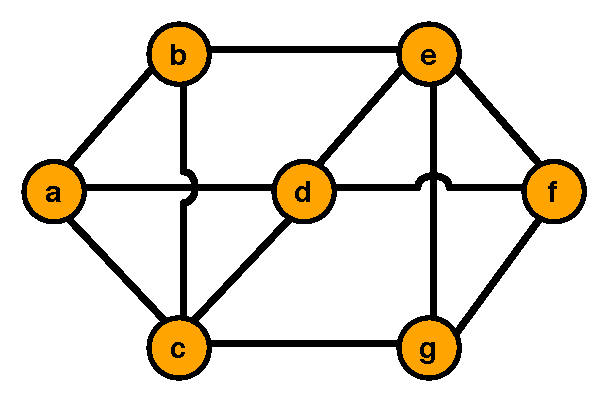
\includegraphics[scale=0.7]{graph_mst.pdf} 
\end{center}
\end{figure}
% ----------

	% YOUR SOLUTION HERE
i) Giving the edges weights: \\
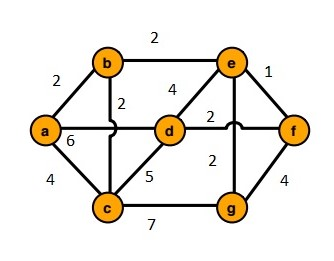
\includegraphics[scale=0.7]{snapegraph.jpg} 

Using Jarnik/Prim's Algorithm \\
Starting at vertex b: choose minimum edge. (All adjacent edges have the same weight, so we can chose any) \\
\hspace*{30mm} $b --> c$ = 2 \\
\hspace*{30mm} $b --> a$ = 2 \\
\hspace*{30mm} $b --> e$ = 2 \\
Choosing fourth minimum edge: \\
\hspace*{30mm} $e --> f$ = 1 \\
Choosing fifth minimum edge: \\
\hspace*{30mm} $e --> g$ = 2 \\
Choosing sixth minimum edge: \\
\hspace*{30mm} $e --> d$ = 4\\
So, all the vertices are covered and the minimum weight of the minimum spanning tree is $((b,c),(b,a),(b,e),(e,f),(e,g),(e,d))$ = 2 + 2 + 2 + 1 + 2 + 4 = 13 \\

Using Kruskal's Algorithm \\
Choosing the smallest edge in the graph: \\
\hspace*{30mm} $e --> f$ = 1 \\
Choosing next smallest from e or f vertex: \\
\hspace*{30mm} $e --> g$ = 2 \\
Choosing next smallest from e, f, and g \\
\hspace*{30mm} $e --> b$ = 2 \\
Choosing next smallest from e, f, g, and b \\
\hspace*{30mm} $b --> a$ = 2 \\
Choosing next smallest from e, f, g, b, and a \\
\hspace*{30mm} $b --> c$ = 2 \\
Choosing next smallest from e, f, g, b, a, c\\
\hspace*{30mm} $e --> d$ = 4 \\
So, all the vertices are covered and the minimum spanning tree of Kruskal's algorithm is $((e,f), (e,g), (e,b), (b,a), (b,c),(e,d))$ = 1 + 2 + 2 + 2 + 4 = 11\\
\\Using Boruvka's Algorithm \\
Initially, it is empty and every vertex is a single component. So for every vertex $v{i}$ find the minimum cost edges that connect vertex $v{i}$ to other components. \\
Vertex $v{i}$ \hspace*{10mm} Minimum cost edge to other component \hspace*{10mm} $w{i}$  \\
a \hspace*{40mm} a,b \hspace*{60mm} 2 \\
b \hspace*{40mm} b,e \hspace*{60mm} 2 \\
c \hspace*{40mm} c,b \hspace*{60mm} 2 \\
d \hspace*{40mm} d,e \hspace*{60mm} 4 \\
e \hspace*{40mm} e,f \hspace*{60mm} 1 \\
f \hspace*{40mm} f,e \hspace*{60mm} (already in) \\
g \hspace*{40mm} g,e \hspace*{60mm} 2 \\
So, the minimum spanning tree becomes (a-b, b-e, c-b,d-e,e-f,g-e)\\
Combining vertices which are connected to each other, \\
\hspace*{10mm} ((a,b,e,f), (c,b), (g,e), (d,e)) = (2+2+1) + 2 + 2 + 4 = 13\\

iii) order edges are added: \\
Jarnik/Prim's: b $->$ ((b,c),(b,a), (b,e), (e,f), (e,g), (e,d)) = 13 \\
Kruskal's: ((e,f), (e,g), (e,b), (b,a), (b,c), (e,d)) = 11 \\
Boruvka's: ((a,b,e,f), (c,b), (g,e), (d,e)) = 13





\\PDFs of images are attached. 
	

	
\end{enumerate}


\end{document}

